\section*{五、数据处理}
\subsection*{1、定标}
在扫描周期0.2ms下,CCD波形一帧对应于示波器上的41个小格。因此,在0.1ms扫描周期下,每格对应的实际空间距离为$\Delta S=\frac{2100}{41*2}*11um=0.3622mm$
\subsection*{2、布拉格衍射的最大衍射效率及带宽}
固定功率情况下,测量数据及当前频率(P为80mA)

%\begin{tabular}{|c|c|c|c|c|c|c|c|c|c|c|c|}
%	\hline 
%	频率${f}_{S}/Hz$&& ||2_fsi||   \\ 
%	\hline 
%	${I}_{1}/$格&& ||2_i1i||   \\ 
%	\hline 
%\end{tabular}
${I}_{0}$ = 19格
可知,当${f}_{c}=||fs1||$时,${I}_{1}$最大,此时有最大衍射效率$\eta=\frac{{I}_{0}}{{I}_{1}}*100\%=\frac{19}{||i1max||}*100\% = ||eta1||$
中心频率光强为$||i1max||$格,当偏转为$\frac{||i1max||}{\sqrt{2}}=||div1||$格时,对应大致频率为||f1||MHz。

所以声光器件的带宽$\Delta {f}_{s}=||fs2||-||fs1||=||f2||MHz$

\begin{figure}[H]
	\centering
	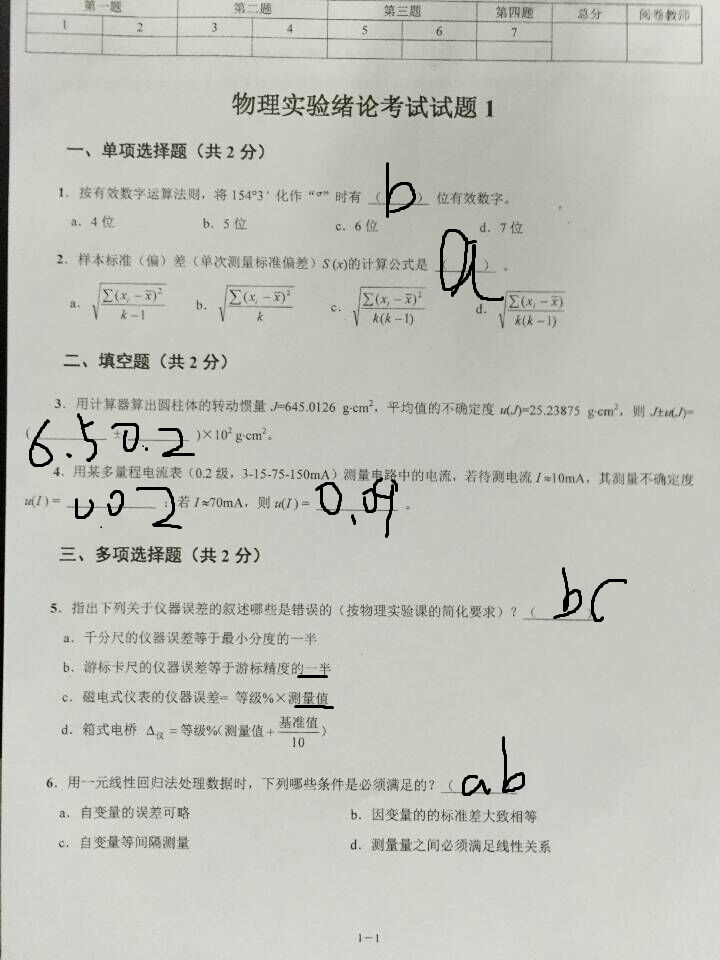
\includegraphics[width=3cm]{Image/1.jpg}
\end{figure}

\subsection*{3、求超声波声速}

\begin{tabular}{|c|c|c|c|c|c|c|c|c|}
	\hline 
	${f}_{s}/$Hz&& ||3_fsi||   \\ 
	\hline 
	间隔小格/div&& ||3_divi||  \\ 
	\hline 
	实际距离D/mm&& ||3_Di||   \\ 
	\hline 
	偏转角度$\phi $/rad&& ||3_phii||   \\ 
	\hline 
	衍射角$\varphi $&& ||3_varphii||   \\ 
	\hline 
\end{tabular} 

以上偏转角为空气中的测量结果,按n =$||3_n||$换算


$\frac{\mathrm{sin}\varphi }{\mathrm{sin}\phi }=\frac{1}{n}$,算出$\varphi$填入上表

根据式$\varphi =\frac{{\lambda }_{0}{f}_{s}}{n{v}_{s}}$得

${f}_{s}=\frac{n{v}_{\delta }}{{\lambda }_{0}}\varphi $

利用一元线性规划,设y = bx+a,y = ${f}_{s}$,x = $\varphi $,

可得b =$||3_b||$ ,$r$ = $||3_r||$ 
可见${f}_{s}$与 $\varphi $与较强线性关系,k置信度高

${V}_{s}=\frac{{\lambda }_{0}{f}_{s}}{n\varphi }=\frac{{\lambda }_{0}}{n}b= \frac{{||3_lambda0 ||}}{||3_n||}||3_b||m/s = ||3_vs1||$
相对误差:$\left|\frac{||3_vs1||-||3_vs2||}{||3_vs2||}\right|*100\%=||3_error||$

\subsection*{4、声光调制}
布拉格衍射,将频率固定在中心频率${f}_{c} = ||4_fc||MHz$

测得:\begin{tabular}{|c|c|c|c|c|c|c|c|c|c|c|c|}
	\hline 
	P(mA)&& ||4_pi||   \\ 
	\hline 
	$I_1/$格&& ||4_i1i||   \\ 
	\hline 
\end{tabular} 

\begin{figure}[H]
	\centering
	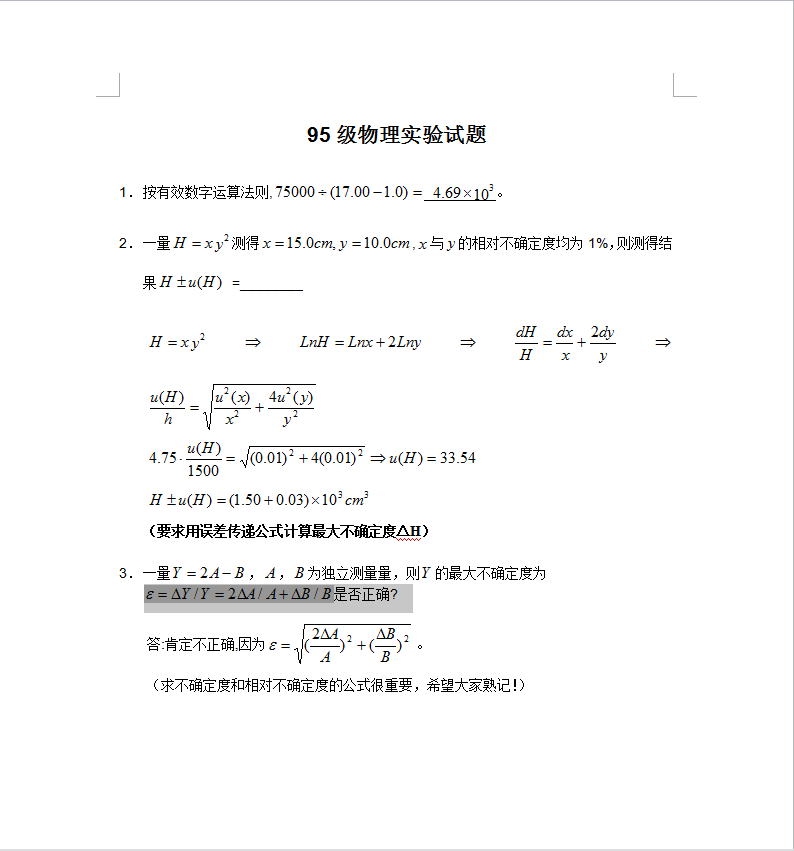
\includegraphics[width=3cm]{Image/2.jpg}
\end{figure}

\subsection*{5、喇曼-纳斯衍射}
(1)$\Delta x=\Delta s*\frac{41}{2} =||5_delta_x||mm$

偏转角$\phi  =arctan\frac{\Delta x}{L} = ||5_phi||$
衍射角$\varphi =\mathrm{arcsin}\left(\frac{\mathrm{sin}\phi }{n}\right) =||5_varphi||rad$
(2)衍射效率
$\eta = \frac{{I}_{1}}{{I}_{0}} = ||5_eta||\%$